\documentclass[12pt, a4paper]{book}

\usepackage[english]{babel}
\usepackage[utf8]{inputenc}
\usepackage{listings}
\usepackage{tikz}

\begin{document}
  \section{Organisation}
  \label{sec:Organisation}
  \section{Demonstration}
  \label{sec:Demonstration}
  \chapter{Foundations}
  \label{chap:Foundations}
  \section{Introduction}
  \label{sec:Introduction}
  \section{Foundations}
  \label{sec:Foundations}

\lstset{morekeywords={if,else,do,while}}
\begin{lstlisting}
stmt  ::= var=expr;
       |  {stmts}
       |  if (bexpr) then stmt else stmt
       |  while (bexpr) do stmt
stmts ::= stmt*
\end{lstlisting}

\begin{verbatim}
expr  ::= nexpr|bexpr|...
nexpr ::= number|var|-nexpr|nexpr+nexpr|...
bexpr ::= true|false|!bexpr|bexpr&&bexpr|...
\end{verbatim}

$nexpr \subset expr$

$bexpr \subset expr$

$(S,\sigma) \longrightarrow (S',\sigma')$

$$\frac{\phi_{1} ... \phi_{n}}{\phi}$$

$$
\frac{(S,\sigma) \longrightarrow (S', \sigma')}
{(\{S\ SS\},\sigma) \longleftarrow (\{S'\ SS\}, \sigma')}
$$

$$
\frac{}
{\ \phi \ }
$$

$$
\frac{}
{(\{ \{ \} \ SS, \sigma \}) \longrightarrow (\{ SS \}, \sigma)}
$$

$$
\frac{\phi_{1} \ldots \phi_{n}}
{\phi}
$$

\begin{eqnarray}
R^{0}   & = & \{\phi \mid \frac{}{\ \phi \ } \exists R\} \\
R^{k+1} & = & R^{k} \cup \{ \phi \mid \frac{\phi_{1} \ldots \phi_{n}}{\phi}
\in R \land \phi_{1}\ldots\phi_{n} \in R^{k} \} \\
R^{*}   & = & \bigcup_{k} R^{k}
\end{eqnarray}

$$
\vdash_{R} \phi \iff \phi \in R^{*}
$$

\paragraph{Assignment V=E;}

$$
\frac{}
{(V=E;,\sigma) \longrightarrow (\{ \}, \sigma [V := \sigma (E)] )}
$$

\paragraph{Sequence \{S SS\}}

$$
\frac{(S,\sigma) \longrightarrow (S',\sigma')}
{(\{ S\ SS \} , \sigma ) \longrightarrow (\{S'\ SS\}, \sigma')}
$$

$$
\frac{}
{(\{ \{ \} SS\}, \sigma) \longrightarrow (\{ SS \}, \sigma)}
$$

\noindent \textbf{Condition} \verb#if# $(B)$ \verb#then# $S_{1}$ \verb#else# $S_{2}$

$$
\frac{}
{(\textrm{if } (B) \textrm{ then } S_{1} \textrm{ else } S_{2}, \sigma) \longrightarrow (S_{1}, \sigma)}
\ \sigma(B)
$$

$$
\frac{}
{(\textrm{if } (B) \textrm{ then } S_{1} \textrm{ else } S_{2}, \sigma) \longrightarrow (S_{2}, \sigma)}
\ \lnot\sigma(B)
$$

\noindent \textbf{Loop} \verb#while# (B) \verb#do# S

$$
\frac{}
{(\textrm{while } (B) \textrm{ do } S, \sigma) \longrightarrow (\{ S \textrm{ while } (B) \textrm{ do } S\}, \sigma)}
\sigma(B)
$$

$$
\frac{}
{(\textrm{while } (B) \textrm{ do } S, \sigma) \longrightarrow (\{ \}, \sigma)}
\lnot\sigma(B)
$$

\paragraph{Runs, Termination, Divergence}

$(S_{0}, \sigma_{0}) \longrightarrow^{*} (S_{k}, \sigma_{k})$ iff there is a
\underline{finite} sequence

$$
(S_{0}, \sigma_{0}) \longrightarrow (S_{1}, \sigma_{1}) \longrightarrow \ldots
\longrightarrow (S_{k}, \sigma_{k})
$$

$(S, \sigma)$ terminates in $\sigma'$ iff $(S, \sigma) \longrightarrow^{*} (\{\}, \sigma')$

$(S_{0}, \sigma_{0}) \longrightarrow^{\omega}$ iff there is an \underline{infinite} sequence

$$
(S_{0}, \sigma_{0}) \longrightarrow (S_{1}, \sigma_{1}) \longrightarrow \ldots
$$

$(S,\sigma)$ diverges iff $(S,\sigma) \longrightarrow^{\omega}$

\paragraph{Semantics: Partial Correctness}

We define the semantics of a program $S$ as a function $[[S]]: \sum \rightarrow 2^{\Sigma}$ \newline

initial store $\rightarrow$ final store \newline

Partial correctness semantics:
$$
[[S]](\sigma) = \{\sigma' \mid (S,\sigma) \longrightarrow^{*} (\{\}, \sigma')\}
$$
where $[[S]](\sigma)$ is the set of possible final stores after executing $S$
from $\sigma$

\paragraph{Semantics (Set-Based Version)}

For convenience, it is useful to define $[[S]]$ on sets of initial states. \newline

For a set of stores $X \subseteq \Sigma$,
$$
[[S]](X) = \bigcup_{\sigma \in X} [[S]](\sigma)
$$

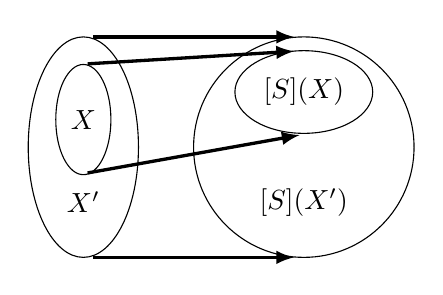
\begin{tikzpicture}[scale=0.7]
  \tikzstyle{suite}=[->,>=stealth’,thick,rounded corners=4pt]

  \draw (1,1) ellipse (1 and 2); % Right big ellipse
  \draw (1,1.5) ellipse (0.5 and 1); % Right little ellipse
  \node (A) at (1, 1.5) {$X$};
  \node (B) at (1, 0.0) {$X'$};
  \draw (5, 1) circle (2); % Right circle
  \draw (5, 2) ellipse (1.25 and 0.75); % Right ellipse in circle
  \node (C) at (5, 2) {$[S](X)$};
  \node (D) at (5, 0) {$[S](X')$};
  \node (E) at (1, 3) {}; % Top-left node
  \node (F) at (5, 3) {}; % Top-right node
  \draw[->,>=latex, very thick] (E)--(F); % Top arrow
  \node (G) at (1,-1) {};
  \node (H) at (5,-1) {};
  \draw[->,>=latex, very thick] (G)--(H); % Bottom arrow
  \node (I) at (0.9, 2.5) {};
  \node (J) at (5, 2.75) {};
  \draw[->,>=latex, very thick] (I)--(J); % Top-ellipse arrow
  \node (K) at (0.9, 0.5) {};
  \node (L) at (5.1, 1.25) {};
  \draw[->,>=latex, very thick] (K)--(L); % Bottom-ellipse arrow
\end{tikzpicture}

\paragraph{Property}: [[S]] is monotonic:

$$
X \subseteq X' \Rightarrow [[S]](X) \subseteq [[S]](X')
$$

\noindent Proof: obvious from definition \newline
Important for convergence of iterative computations

  \chapter{Program Proofs}
  \label{chap:Program Proofs}
  \section{Sequential Programs}
  \label{sec:Sequential Programs}
  \section{Verification Conditions}
  \label{sec:Verification Conditions}
  \section{Procedures}
  \label{sec:Procedures}
  \section{Recursion}
  \label{sec:Recursion}
  \section{Data Structures}
  \label{sec:Data Structures}
  \section{Reactive Programs}
  \label{sec:Reactive Programs}
  \chapter{Program Validation}
  \label{chap:Program Validation}
  \section{State-Based Models}
  \label{sec:State-Based Models}
  \section{Model Checking}
  \label{sec:Model Checking}
\end{document}
